\documentclass[11pt]{article}
\usepackage[a4paper, total={7in, 10in}]{geometry}
\usepackage{amsmath}
\usepackage{graphicx}
\usepackage{hyperref}
\graphicspath{ {./resources/} }
\usepackage[font=small,labelfont=bf]{caption} % Required for specifying captions to tables and figures
\usepackage[T1]{fontenc}
\usepackage[utf8]{inputenc}


\title{Scientific Computing - Interpolation}
\author{Mateusz Pełechaty}
\date{23 October 2022}%
\begin{document}
\maketitle

\section{Exercise}
Write function, which calculates Newton's divided differences for given function.
Function should be named \textit{dividedDifference} and should take two arguments: 
\begin{itemize}
    \item $\vec{x}$ : vector of nodes
    \item $\vec{f}$ : vector of function values at nodes
\end{itemize}
Function should not use two-dimensional array.
\subsection*{Algorithm Description}
Newton's divided differences are defined as follows:
\begin{equation}
    f[x_0, x_1, \dots, x_n] = \frac{f[x_1, x_2, \dots, x_n] - f[x_0, x_1, \dots, x_{n-1}]}{x_n - x_0}\\
\end{equation}
\begin{equation*}
    f[x_i] = f(x_i)
\end{equation*}
We can compute them in one-dimensional array by looping from last to first with the help of formula $(1)$:
\begin{equation*}
\begin{pmatrix}
    f[x_0] \\
    f[x_1] \\
    f[x_2] \\
    \vdots \\
    f[x_{n-1}] \\
    f[x_n] \\
\end{pmatrix}
\rightarrow
\begin{pmatrix}
    f[x_0] \\
    f[x_0,x_1] \\
    f[x_1, x_2] \\
    \vdots \\
    f[x_{n-2},x_{n-1}] \\
    f[x_{n-1}, x_n] \\
\end{pmatrix}
\rightarrow
\begin{pmatrix}
    f[x_0] \\
    f[x_0,x_1] \\
    f[x_0,x_1,x_2] \\
    \vdots \\
    f[x_0 \hdots x_{n-2},x_{n-1}] \\
    f[x_0 \hdots x_{n-1}, x_n] \\
\end{pmatrix}
\end{equation*}
\subsection*{Solutions and tests}
Function with documentation can be found in \textit{src/interpolation.jl}. \\
Tests are in \textit{test/test\_dividedDifference.jl}

\section{Exercise}
Write function which calculates value of polynomial at a given point.
Function should be named \textit{valueNewton} and should take three arguments: 
\begin{itemize}
    \item $\vec{x}$ : vector of nodes
    \item $\vec{f}$ : vector of function values at nodes
    \item t : point at which polynomial should be evaluated
\end{itemize}
Function should compute in $O(n)$ time complexity
\subsection*{Algorithm Description}
Method of computation is based on Horner's rule:
\begin{equation*}
\begin{split}
    p(x) &= a_0 + a_1(x-x_0) + a_2(x-x_0)(x-x_1) + \dots + a_n(x-x_0)(x-x_1)\dots(x-x_{n-1})\\
     &= a_0 + (a_1 + (a_2 + \dots (a_{n-1} + (a_n \cdot (x-x_{n-1}))(x-x_{n-2}))\dots)(x-x_0)
\end{split}
\end{equation*}
We start from the innermost term, add coefficient and multiply by ${x-x_i}$ till we reach the outermost term.
\subsection*{Solutions and tests}
Function with documentation can be found in \textit{src/interpolation.jl}.\\
Tests are in \textit{test/test\_valueNewton.jl}
\section{Exercise}
Write a function that can compute coefficients of a polynomial in general form by using Newton's divided differences.
Function should be named \textit{general} and should take two arguments:
\begin{itemize}
    \item $\vec{x}$ : vector of nodes
    \item $\vec{f}$ : vector of function values at nodes
\end{itemize}
Function should compute in $O(n^2)$ time complexity

\subsection*{Solutions and tests}
Function with documentation can be found in \textit{src/interpolation.jl}.\\
Tests are in \textit{test/test\_general.jl}
\subsection*{Algorithm Description}
We are going to multiplicate all terms in a polynomial in Newton's form in a smart way.\\
Assume we have $\vec{x}[0..n-1]$ and \textit{divided differences} $\vec{c}[0..n-1]$\\
Let $q_k = \prod^{k-1} _{i=0}(x-x_i)$, $q_0 = 1$\\
Now we can write interpolated polynomial in Newton form as
\begin{equation*}
    f(x) = \sum^n_{i=0}{c_i \cdot q_i(x)}
\end{equation*}
Let's start by computing every $q_i$. From $q_i = q_{i-1} \cdot (x-x_{i-1})$ 
we can figure out following coefficients (\textbf{C}) table and thus, the relation
\begin{table}[!ht] 
    \centering
    \begin{tabular}{|c|c|c|c|c|}
    \hline
        \textbf{C} & \textbf{$q_0$} & \textbf{$q_1$} & \textbf{$q_2$} & \textbf{$q_3$} \\ \hline
        \textbf{$a_0$} & $1$ & $-x_1$ & $x_1 \cdot x_2$ & $- x_1 \cdot x_2 \cdot x_3$ \\ \hline
        \textbf{$a_1$} & 0 & $1$ & $-x_1 - x_2$ & $x_1 \cdot x_2 - x_3 \cdot (-x_1 - x_2)$ \\ \hline
        \textbf{$a_2$} & 0 & 0 & $1$ & $- x_1 - x_2 - x_3$ \\ \hline
        \textbf{$a_3$} & 0 & 0 & 0 & $1$ \\ \hline
    \end{tabular}
\end{table}
\begin{equation*}
    C[q_i, a_i] = C[q_{i-1}, a_{i-1}] - C[q_{i-1}, a_i] \cdot x_{i+1}
\end{equation*}
Note that to compute $a_i$ of $f(x)$ we need to make scalar product of row $a_i$ in $C$ and $\vec{c}$
\section{Exercise}
Write a function that will interpolate given function on a given interval using Newton's interpolation formula.
Then it should plot the function and its interpolation. Function should be named \textit{drawInterpolation} and should take four arguments:
\begin{itemize}
    \item $f$ : anonymous function to interpolate 
    \item $[a, b]$ : left and right bounds of interval
    \item $n$ : Interpolated polynomial's degree
\end{itemize}
\subsection*{Solutions and tests}
Function with documentation can be found in \textit{src/interpolation.jl}\\
Tests are in \textit{test/test\_drawInterpolation.jl}
\section{Exercise}
Test function \textit{drawInterpolation} with the following arguments:
\begin{itemize}
    \item $e^x, [0, 1], n=5,10,15$
    \item $x^2 \cdot \sin x, [-1, 1], n=5,10,15$
\end{itemize}
\subsection*{Solutions and results}
Solution can be found in \textit{src/ex5/main.jl}. Plots can be found in \textit{src/results/}:
\subsection*{Results} 
\begin{figure}[h]
    \centering
    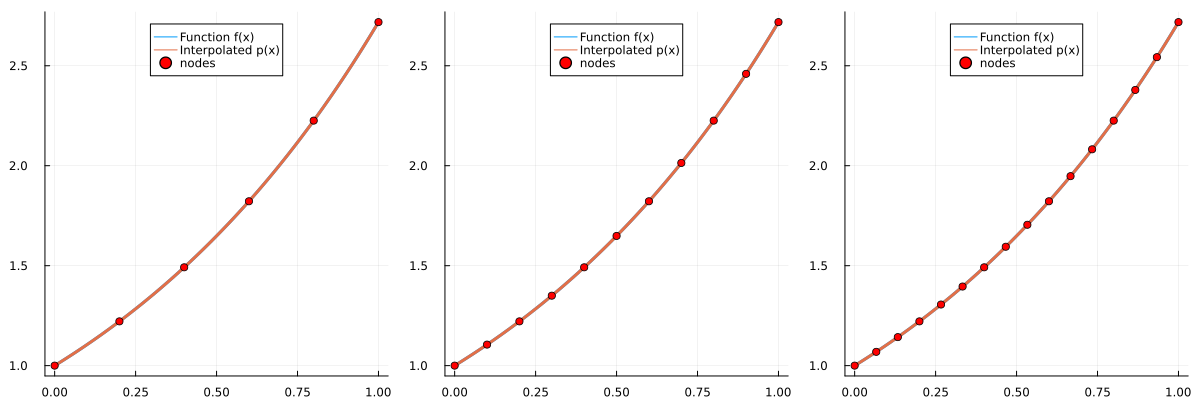
\includegraphics[width=1\textwidth]{ex5_plot1.png}
    \caption{Interpolation of $f(x)=exp(x)$, $[a,b] = [0,1]$ and $n = [5,10,15]$}
\end{figure}
\begin{figure}[h]
    \centering
    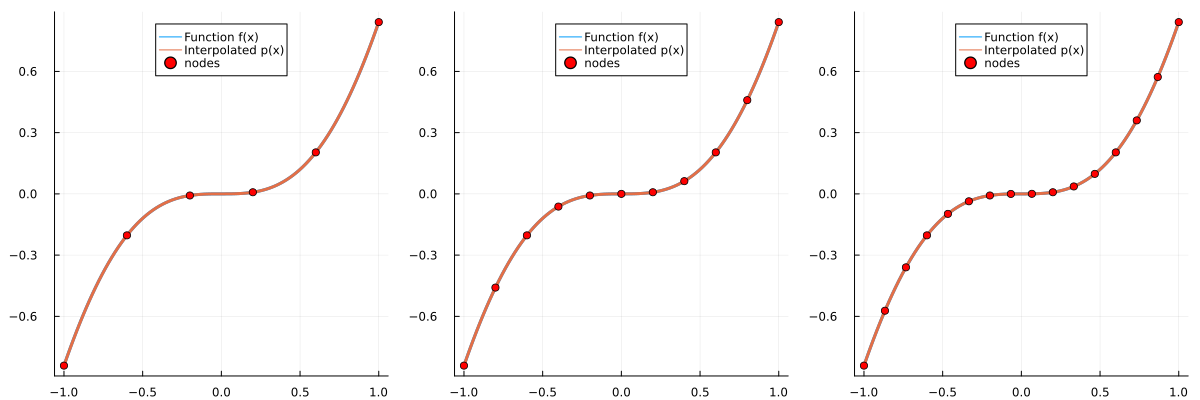
\includegraphics[width=1\textwidth]{ex5_plot2.png}
    \caption{Interpolation of $f(x)=x^2 \cdot sin(x)$, $[a,b] = [-1,1]$ and $n = [5,10,15]$}
\end{figure}
\subsection*{Conclusion}
We can see that there is no visible difference between interpolation and function itself. 
This is due to two reasons:
\begin{itemize}
    \item We are interpolating on a small interval
    \item We can bound maximum of $\frac{f^{(n+1)}(\xi)}{(n+1)!}$
    \item $f$ is smooth and behaves well. One could say that $f$ is \textit{preety}
\end{itemize}
\section{Exercise}
Spot \textit{discrepancy phenomena} by testing function \textit{drawInterpolation} with the following arguments:
\begin{itemize}
    \item $|x|, [-1, 1], n=5,10,15$
    \item $\frac{1}{1+x^2}, [-5, 5], n=5,10,15$; so called Runge's phenomenon
\end{itemize}
\subsection*{Solutions}
Solution can be found in \textit{src/ex6/main.jl}. Plots can be found in \textit{src/results/}
\subsection*{Results}
\begin{figure}[h]
    \centering
    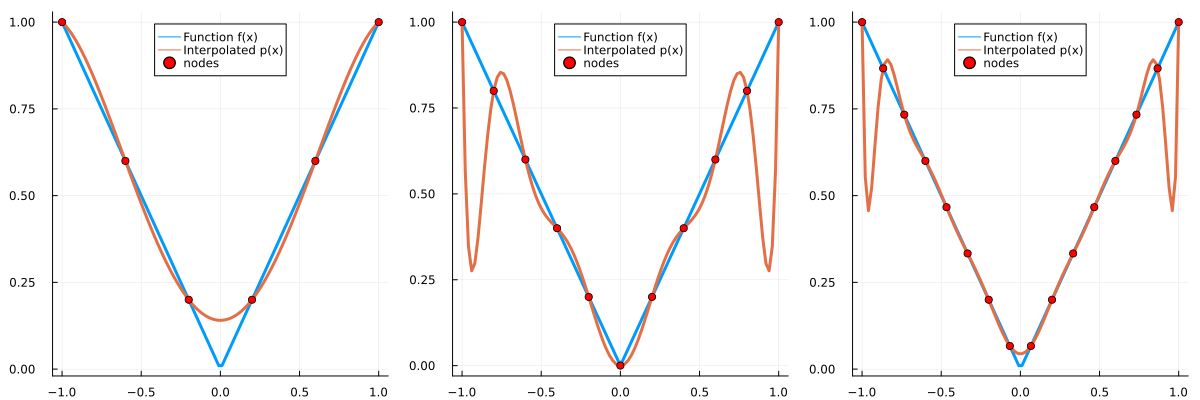
\includegraphics[width=1\textwidth]{ex6_plot1.png}
    \caption{Interpolation of $f(x)=|x|$, $[a,b] = [-1,1]$ and $n = [5,10,15]$}
\end{figure}
\begin{figure}[h]
    \centering
    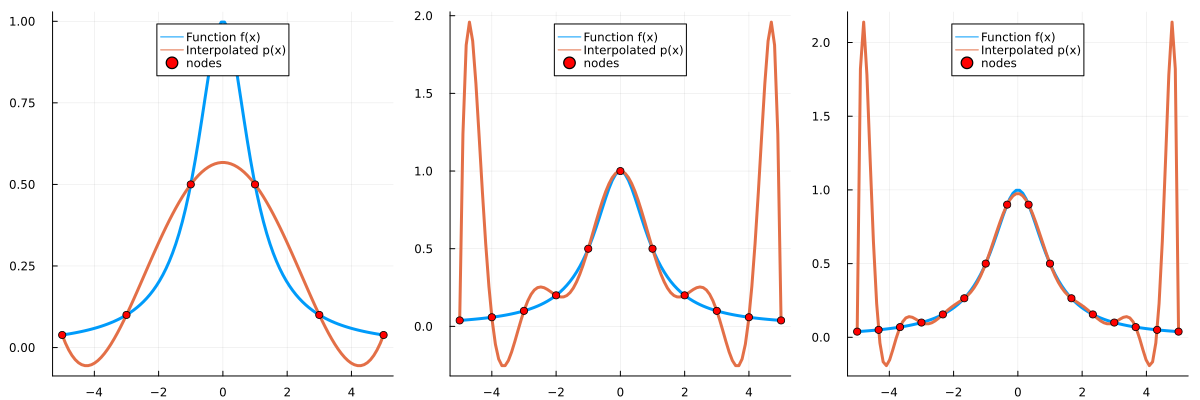
\includegraphics[width=1\textwidth]{ex6_plot2.png}
    \caption{Interpolation of $f(x)=1/(1+x^2)$, $[a,b] = [-5,5]$ and $n = [5,10,15]$}
\end{figure}
\subsection*{Conclusion}
We can see that there is visible difference between interpolation and function itself.
When amount of nodes gets bigger, we can see that magnitude of the oscillations in the interpolation is increased.
We can analyse the error formula to see why this happens:
\begin{equation*}
    f(x) - p(x) = \frac{f^{(n+1)}(\xi)}{(n+1)!} \cdot \Pi^n_{i=0}(x-x_i)
\end{equation*}
where $\xi$ is some point between $a$ and $b$\\
Even though I can't exactly say why this phenomena happens, 
I can spot that when when points are equidistanced, then for $x = a + \frac{b-a}{2n}$
\begin{equation*}
    \Pi^n_{i=0}{(x-x_i)} = (\frac{b-a}{2n})^2 \cdot \Pi ^n _{i=2}(i\cdot\frac{b-a}{n} + \frac{b-a}{2n}) 
    = (\frac{b-a}{2n})^{n+1} + (\frac{b-a}{n})^{n-1} \cdot n! \\
\end{equation*}
Let's calculate what happens when $ n \to \infty $  
\begin{equation*}
    \lim_{n \to \infty} \Pi^n_{i=0}{(x-x_i)} = \lim_{n \to \infty} (\frac{b-a}{n})^{n-1} \cdot n! = \lim_{n \to \infty}  (\frac{b-a}{n})^{n-1} \cdot \sqrt{2\pi n} \cdot (\frac{n}{e})^n = \lim_{n \to \infty} (\frac{b-a}{e})^{n-1} \cdot n\sqrt{n} \cdot e^{-1}
\end{equation*}
We can see that if $b-a \geq e $ then the product grows exponentially. It may show the reason why the oscillations are growing at the edges of interval.
To fully prove that the error grows exponentially, we would have to also grasp $f^{(n+1)}(\xi)$, to which I have no idea how to do.
\end{document} 